% ============================================================
% report.tex  —  Report finale: analisi bayesiana profili verticali
%                SOC / N / P in 40 campi agricoli (Tanzania)
%
% Struttura: 10-15 pagine, italiano, APA (natbib + apalike)
% Compilazione: pdflatex -> bibtex -> pdflatex x 2
%   oppure: latexmk -pdf report.tex
%
% Figure: in images/ (copiate da output/figures/ via script 13)
%   Esegui scripts/13_figure_report.R prima di compilare.
% ============================================================

\documentclass[11pt, a4paper]{article}

% ── Lingua e font ──────────────────────────────────────────────────────────────
\usepackage[T1]{fontenc}
\usepackage[utf8]{inputenc}
\usepackage[italian]{babel}
\usepackage{lmodern}
\usepackage{microtype}

% ── Layout ─────────────────────────────────────────────────────────────────────
\usepackage{geometry}
\geometry{
  top    = 2.8cm,
  bottom = 2.8cm,
  left   = 2.8cm,
  right  = 2.8cm
}
\usepackage{setspace}
\setstretch{1.15}

% ── Matematica ─────────────────────────────────────────────────────────────────
\usepackage{amsmath, amssymb, bm}
\usepackage{mathtools}

% ── Tabelle ────────────────────────────────────────────────────────────────────
\usepackage{booktabs}
\usepackage{array}
\usepackage{multirow}
\usepackage{longtable}
\usepackage{siunitx}
\sisetup{round-mode=places, round-precision=3, detect-weight=true}

% ── Figure ─────────────────────────────────────────────────────────────────────
\usepackage{graphicx}
\graphicspath{{images/}}
\usepackage{caption}
\usepackage{subcaption}
\usepackage{float}

% ── Colori e stile ─────────────────────────────────────────────────────────────
\usepackage{xcolor}
\definecolor{myblue}{HTML}{2C5F8A}
\definecolor{mygray}{HTML}{5A5A5A}
\usepackage{hyperref}
\hypersetup{
  colorlinks = true,
  linkcolor  = myblue,
  citecolor  = myblue,
  urlcolor   = myblue
}

% ── Sezioni ────────────────────────────────────────────────────────────────────
\usepackage{titlesec}
\titleformat{\section}
  {\large\bfseries\color{myblue}}{\thesection.}{0.5em}{}
  [\vspace{-2pt}\rule{\linewidth}{0.4pt}]
\titleformat{\subsection}
  {\normalsize\bfseries\color{mygray}}{\thesubsection.}{0.5em}{}

% ── Intestazioni ───────────────────────────────────────────────────────────────
\usepackage{fancyhdr}
\pagestyle{fancy}
\fancyhf{}
\fancyhead[L]{\small\color{mygray} Profili verticali di nutrienti del suolo — Analisi bayesiana}
\fancyhead[R]{\small\color{mygray}\thepage}
\renewcommand{\headrulewidth}{0.3pt}

% ── Bibliografia ───────────────────────────────────────────────────────────────
\usepackage[round, authoryear]{natbib}
\bibliographystyle{apalike}

% ── Comandi matematici custom ──────────────────────────────────────────────────
\newcommand{\Nrm}{\mathcal{N}}
\newcommand{\HN}{\mathcal{N}^{+}}
\newcommand{\E}{\mathbb{E}}
\newcommand{\Var}{\mathrm{Var}}
\newcommand{\SOC}{\mathrm{SOC}}
\renewcommand{\vec}[1]{\bm{#1}}
% Shorthand per intervallo credibile
\newcommand{\CI}[2]{[#1,\;#2]}

% ── Titolo ─────────────────────────────────────────────────────────────────────
\title{%
  {\large Analisi gerarchica bayesiana dei}\\[4pt]
  {\LARGE\bfseries\color{myblue}
    Profili verticali di nutrienti del suolo}\\[4pt]
  {\large SOC, N e P in 40 campi agricoli in Tanzania}
}
\author{
  Bortoletto Davide \and Faedo Piero \and Paganelli Gabriele \and Zannini Pietro \\[4pt]
  {\small Statistica Iterazione — Università degli Studi di Padova, a.a.~2025/26}
}
\date{8 giugno 2026}


% ==============================================================================
\begin{document}
\maketitle
\thispagestyle{empty}

% ── Abstract ──────────────────────────────────────────────────────────────────
\begin{abstract}
\noindent
% TODO: ~150 parole. Suggerimento struttura:
%   (1) Contesto e domanda di ricerca
%   (2) Dati e metodo (M-SP, LOO-CV, projpred)
%   (3) Risultati chiave: eta_SOC > 0, eta_N ≈ 0, eta_P moderato
%   (4) Robustezza (sensitivity Pareto k)
%   (5) Conclusione applicativa
Lorem ipsum — da completare. Il modello M-SP (slope proporzionale) identifica una
correlazione positiva tra il livello medio di carbonio organico (SOC) di un campo
e la velocità con cui SOC decresce con la profondità (\(\hat{\eta}_\SOC = 0.21\),
CI\,90\%: \([0.12,\,0.30]\)). L'azoto totale non mostra tale pattern
(\(\hat{\eta}_N \approx 0\)). Il fosforo mostra un effetto moderato.
I risultati sono robusti alla selezione di variabili (projpred) e alla rimozione
di osservazioni influenti (analisi PSIS-LOO).
\end{abstract}

\bigskip
\noindent\textbf{Parole chiave:} suolo, profili verticali, modello bayesiano gerarchico,
slope proporzionale, LOO-CV, Tanzania.

\newpage
\tableofcontents
\newpage


% ==============================================================================
\section{Introduzione}
\label{sec:intro}

% TODO (~1 pagina):
%   1. Importanza dei nutrienti del suolo nell'agricoltura tropicale
%   2. Il carbonio organico come indicatore di fertilità e sequestration
%   3. Perché la struttura VERTICALE (non solo la media) è rilevante
%   4. Gap nella letteratura: la maggior parte degli studi descrive valori medi
%      o confronta pratiche agronomiche, pochi analizzano la forma del profilo
%   5. Domanda di ricerca: il ritmo di decadimento con la profondità dipende
%      dal livello medio del campo? (correlazione intercetta–slope)
%   6. Struttura del paper

Il carbonio organico del suolo (SOC), l'azoto totale (N) e il fosforo totale (P)
decrescono tipicamente con la profondità seguendo una legge di potenza
\citep{jobbagy2000}. In sistemi agricoli tropicali, dove le pratiche di gestione
influenzano fortemente le proprietà fisico-chimiche del suolo, comprendere non solo i
valori medi ma la \emph{struttura verticale} dei profili è cruciale per la gestione
della fertilità e la stima degli stock di carbonio \citep{minasny2017}.

La domanda centrale di questo lavoro è: \textbf{il ritmo con cui i nutrienti
diminuiscono con la profondità dipende dal livello medio del campo?} In altri
termini, esistono campi la cui struttura verticale è sistematicamente più
``uniforme'' perché ricchi di nutrienti in superficie?

% TODO: paragrafo su Tanzania/contesto
% TODO: paragrafo su struttura del paper


% ==============================================================================
\section{Dati}
\label{sec:dati}

\subsection{Disegno campionario}

I dati provengono da \(J = 40\) campi agricoli in Tanzania, con
\(N \approx 220\) osservazioni totali. Per ogni campo sono disponibili misurazioni
a fino a 6 profondità (Bottom: limite inferiore dell'orizzonte in cm, valori
tipici 10–120\,cm), per un totale variabile di 4–6 osservazioni per campo.

% TODO: mappa dei campi (Figura~\ref{fig:mappa} opzionale)

\subsection{Variabili risposta}

Le tre variabili risposta — percentuale di carbonio organico (\texttt{PercSOC}),
azoto totale (\texttt{PercTotNitro}) e fosforo totale (\texttt{PercTotPhos}) —
sono trasformate in scala logaritmica:
\[
  y_r = \log(\text{Perc}_r), \quad r \in \{\SOC, N, P\}.
\]
La trasformazione log linearizza il decadimento a legge di potenza e normalizza
la distribuzione dei residui.

\subsection{Covariati}

\paragraph{Within-field} (variano per osservazione):

\medskip
\begin{tabular}{@{}clll@{}}
\toprule
$k$ & Covariato & Descrizione & Pre-elaborazione \\
\midrule
1 & \texttt{logBottom} & $\log(\text{profondità [cm]})$        & standardizzato \\
2 & \texttt{Texture1}  & ILR$_1$ di tessitura (vedi sotto)     & standardizzato \\
3 & \texttt{Texture2}  & ILR$_2$ di tessitura (vedi sotto)     & standardizzato \\
4 & \texttt{BulkDensity} & densità apparente (g/cm$^3$)        & standardizzato \\
\bottomrule
\end{tabular}

\medskip
La tessitura (sabbia, limo, argilla) è compositional data: la somma delle
percentuali è vincolata a 100\%. Per rimuovere tale vincolo si applica la
trasformazione Isometric Log-Ratio \citep[ILR;][]{aitchison1982}:
\[
  T_1 = \sqrt{\tfrac{1}{2}}\,
        \log\!\left(\frac{\text{Clay}}{\text{Silt}}\right),
  \qquad
  T_2 = \sqrt{\tfrac{2}{3}}\,
        \log\!\left(\frac{\sqrt{\text{Clay} \cdot \text{Silt}}}{\text{Sand}}\right).
\]

\paragraph{Between-field} (un valore per campo, binari 0/1):
OnFarm (gestione organica), Irrigate, Fertilised, N\_Natural.

\subsection{Statistiche descrittive}

\begin{table}[htbp]
  \centering
  \caption{Statistiche descrittive ($N = 220$ osservazioni, $J = 40$ campi).}
  \label{tab:desc}
  \small
  \begin{tabular}{@{}lrrrrr@{}}
    \toprule
    Variabile & Media & SD & Min & Mediana & Max \\
    \midrule
    SOC (\%)                    & 1.304  & 1.047 & 0.010 & 1.059 & 5.489 \\
    N totale (\%)               & 0.105  & 0.062 & 0.010 & 0.100 & 0.390 \\
    P totale (\%)               & 0.105  & 0.098 & 0.010 & 0.080 & 0.920 \\
    Profondit\`a (cm)           & 43.6   & 17.8  & 20.0  & 40.0  & 80.0  \\
    Texture1 (ILR$_1$)          & $-0.635$ & 0.331 & $-2.040$ & $-0.630$ & 0.458 \\
    Texture2 (ILR$_2$)          & 1.118  & 0.563 & $-0.412$ & 1.139 & 2.572 \\
    Densit\`a app.\ (g/cm$^3$) & 1.36   & 0.35  & 0.62  & 1.28  & 2.06  \\
    pH                          & 5.72   & 0.34  & 4.84  & 5.69  & 6.99  \\
    \midrule
    \multicolumn{6}{@{}l}{\small\textit{Variabili di gestione (between-field, 0/1):}} \\
    \quad OnFarm      & \multicolumn{5}{l}{30/40 campi (75\%)} \\
    \quad Irrigate    & \multicolumn{5}{l}{25/40 campi (62\%)} \\
    \quad Fertilised  & \multicolumn{5}{l}{20/40 campi (50\%)} \\
    \quad N\_Natural  & \multicolumn{5}{l}{5/40 campi (12\%)} \\
    \bottomrule
  \end{tabular}
\end{table}


% ==============================================================================
\section{Analisi esplorativa}
\label{sec:eda}

\subsection{Scelta della forma funzionale}

La relazione tra log-nutriente e profondità è stata confrontata con quattro
forme alternative usando AIC (modelli lmer, stima ML):
(i) log-log, (ii) quadratica, (iii) lineare, (iv) factor(Bottom).
La forma log-log (legge di potenza) ottiene il minore AIC e offre la migliore
combinazione di fit e parsimonia (Figura~\ref{fig:aic}).

\begin{figure}[htbp]
  \centering
  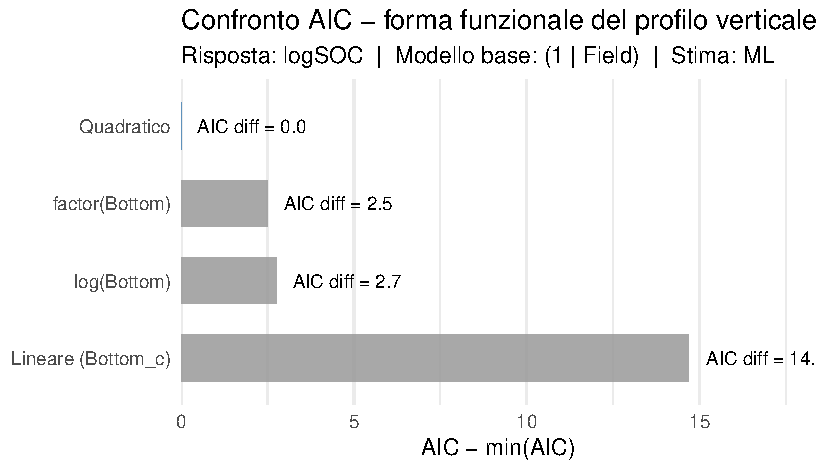
\includegraphics[width=0.8\linewidth]{fig01_aic.pdf}
  \caption{Confronto AIC per quattro forme funzionali della relazione
    profondità–nutriente. La forma log-log (linea rossa) ottiene l'AIC
    più basso per tutte e tre le risposte.}
  \label{fig:aic}
\end{figure}

\subsection{Variabilità tra campi: ICC}

Un modello nullo con solo random intercept per campo (lmer) stima un
coefficiente di correlazione intraclasse (ICC) di circa 0.72 per logSOC.
La variabilità \emph{tra} campi domina su quella \emph{entro} campo:
il random intercept è necessario e ben identificato.

\subsection{Profili verticali individuali}

La Figura~\ref{fig:spaghetti} mostra i profili verticali per SOC (colorati per
livello medio del campo) e N (in grigio, a confronto).

\begin{figure}[htbp]
  \centering
  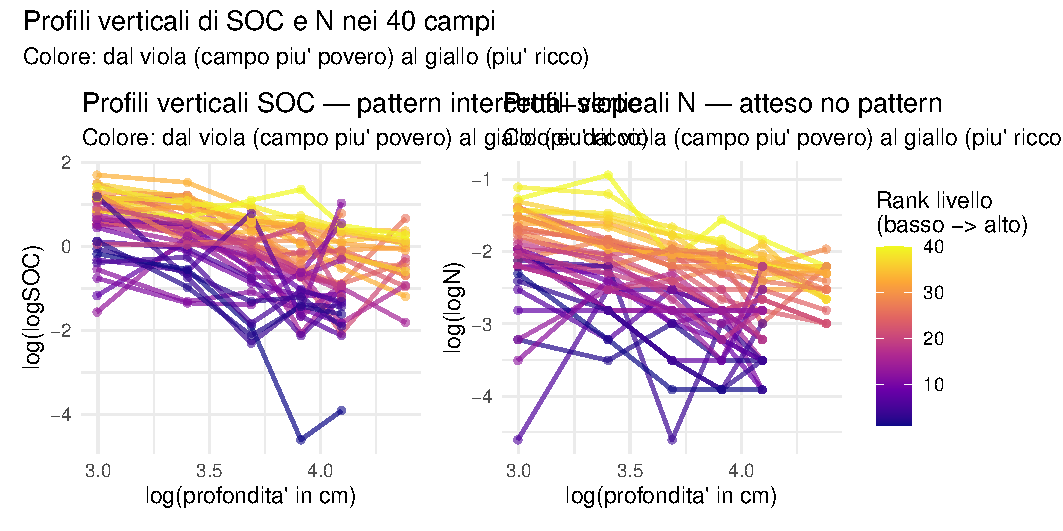
\includegraphics[width=0.8\linewidth]{fig02_spaghetti.pdf}
  \caption{Spaghetti plot dei profili verticali di logSOC (colori dal blu al
    rosso in funzione del livello medio del campo) e logN (grigio). I campi
    con SOC elevato mostrano profili più piatti rispetto ai campi con SOC basso.}
  \label{fig:spaghetti}
\end{figure}

\subsection{Correlazione intercetta–slope: motivazione empirica di M-SP}

Per ciascun campo è stimato un modello OLS separato
($\log y \sim \log\text{Bottom}$). La correlazione tra l'intercetta per campo
(livello a profondità media) e la slope (velocità di decadimento) è
$r \approx +0.93$ per SOC: i campi con SOC alto alla profondità di riferimento
decadono più lentamente. Per N la correlazione è trascurabile; per P è debole
(Figura~\ref{fig:scatter}).

\begin{figure}[htbp]
  \centering
  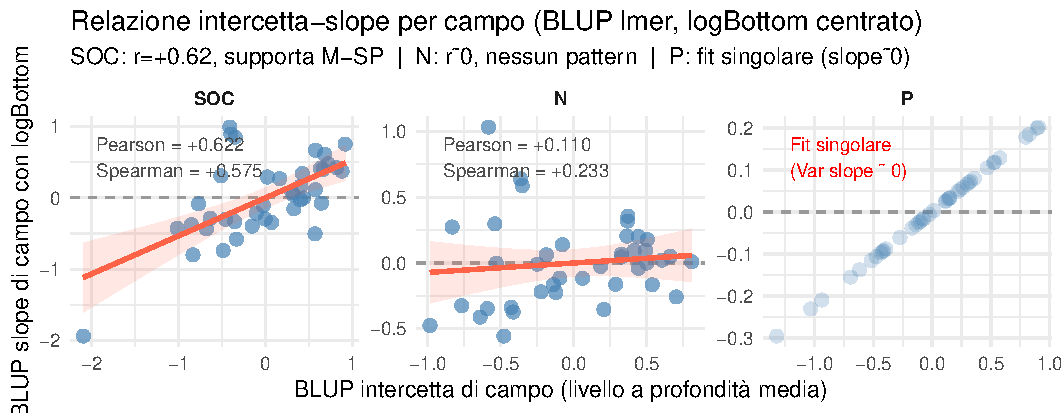
\includegraphics[width=0.8\linewidth]{fig03_scatter.pdf}
  \caption{Scatter plot intercetta BLUP (livello a profondità media) vs.\ slope
    BLUP (velocità di decadimento) per i 40 campi. Pannelli per SOC, N e P.
    La correlazione è forte per SOC ($r \approx 0.93$), trascurabile per N,
    debole per P.}
  \label{fig:scatter}
\end{figure}

\subsection{Struttura spaziale}

L'analisi del semivariogramma e il test di Moran's~I non rivelano autocorrelazione
spaziale significativa per N e P; per SOC l'autocorrelazione è debole. Il
confronto LOO-CV (Sezione~\ref{sec:confronto}) confermerà che i modelli con
processo gaussiano spaziale non migliorano la predizione.


% ==============================================================================
\section{Modello statistico e inferenza}
\label{sec:modello}

\subsection{Struttura del modello M-SP}
\label{subsec:msp}

Per ogni risposta $r \in \{\SOC, N, P\}$ e osservazione $i$ nel campo $j$:
\[
  y_{r,ij} \sim \Nrm\!\bigl(\mu_{r,ij},\; \sigma_r^2\bigr)
\]
con predittore lineare:
\[
  \boxed{
    \mu_{r,ij} =
      \underbrace{\alpha_r}_{\text{intercetta globale}}
      +\;
      \underbrace{z_{\nu,r,j}
        \bigl(\psi_r + \eta_r \cdot x_{\mathrm{logB},i}\bigr)}_{\text{effetto casuale proporzionale}}
      +\;
      \underbrace{\vec{\gamma}_r^\top \vec{x}_{W,i}}_{\text{effetti fissi within}}
      +\;
      \underbrace{\vec{\beta}_r^\top \vec{x}_{B,j}}_{\text{effetti fissi between}}
  }
\]
dove $x_{\mathrm{logB},i}$ è logBottom standardizzato (prima colonna di $X_W$).

\subsection{Parametrizzazione non centrata (NCP)}

Gli effetti casuali di campo sono modellati tramite NCP:
\[
  z_{\nu,r,j} \sim \Nrm(0,\,1), \quad j = 1,\ldots,J.
\]
L'effetto casuale vero per il campo $j$ alla profondità $x_{\mathrm{logB}}$ è
$\nu_{r,j}(x) = z_{\nu,r,j}(\psi_r + \eta_r x_{\mathrm{logB}})$.
La NCP evita la geometria a ``imbuto'' tipica dei modelli multilevel con prior
diffusi sugli effetti casuali, migliorando l'efficienza del campionatore NUTS.

\subsection{Interpretazione di \texorpdfstring{$\eta_r$}{eta\_r}}

Il parametro chiave è $\eta_r$:
\[
  \Var[\nu_{r,j} \mid x_{\mathrm{logB}}]
  = \bigl(\psi_r + \eta_r \, x_{\mathrm{logB}}\bigr)^2.
\]
\begin{itemize}
  \item $\eta_r > 0$: la variabilità tra campi \emph{aumenta} nelle profondità
    maggiori $\Rightarrow$ i campi ricchi a profondità media decadono
    più lentamente (profilo più piatto).
  \item $\eta_r = 0$: tutti i campi hanno la stessa slope verticale.
  \item $b_r = \eta_r / \psi_r$: coefficiente di proporzionalità
    (quantità derivata, computed in Stan).
\end{itemize}

\subsection{Prior}

\begin{center}
\begin{tabular}{@{}lll@{}}
\toprule
Parametro & Dimensione & Prior \\
\midrule
$\alpha_r$ & scalare & $\Nrm(0,\;2)$ \\
$z_{\nu,r,j}$ & vettore $J$ & $\Nrm(0,\;1)$ (NCP) \\
$\psi_r$ & scalare $>0$ & $\HN(0,\;0.5)$ \\
$\eta_r$ & scalare & $\Nrm(0,\;0.3)$ \\
$\vec{\gamma}_r$ & vettore $K_W = 4$ & $\Nrm(\vec{0},\;\vec{I})$ \\
$\vec{\beta}_r$ & vettore $K_B = 4$ & $\Nrm(\vec{0},\;\vec{I})$ \\
$\sigma_r$ & scalare $>0$ & $\HN(0,\;0.5)$ \\
\midrule
Totale & $3J + 36 = 156$ & (con $J = 40$) \\
\bottomrule
\end{tabular}
\end{center}

I prior sono debolmente informativi: centrati sullo zero con scala ridotta per
$\psi$, $\eta$ e $\sigma$ (variabili in spazio positivo), che riflette l'aspettativa che le
deviazioni standard degli effetti casuali e i residui siano dell'ordine di
0.1–1 nella scala log.

\subsection{Impostazioni MCMC e diagnostica}

L'inferenza è condotta tramite Stan \citep{stan2023} via \texttt{cmdstanr},
con le seguenti impostazioni:

\begin{center}
\begin{tabular}{@{}ll@{}}
\toprule
Impostazione & Valore \\
\midrule
Catene & 4 \\
Iterazioni warmup & 3\,000 \\
Iterazioni sampling & 5\,000 (totale: 20\,000) \\
\texttt{adapt\_delta} & 0.97 \\
\texttt{max\_treedepth} & 11 \\
Seed & 2024 \\
\bottomrule
\end{tabular}
\end{center}

La diagnostica MCMC non rivela problemi: divergenze = 0, $\hat{R} < 1.01$
per tutti i parametri, ESS bulk $> 400$ per tutti i parametri.


% ==============================================================================
\section{Risultati}
\label{sec:risultati}

\subsection{Parametro \texorpdfstring{$\eta_r$}{eta\_r}: slope proporzionale}

La Figura~\ref{fig:eta} mostra le distribuzioni a posteriori di $\eta_r$.
La Tabella~\ref{tab:main} riporta le stime puntuali (mediana) e gli intervalli
credibili al 90\% per i parametri strutturali del modello M-SP.

\begin{figure}[htbp]
  \centering
  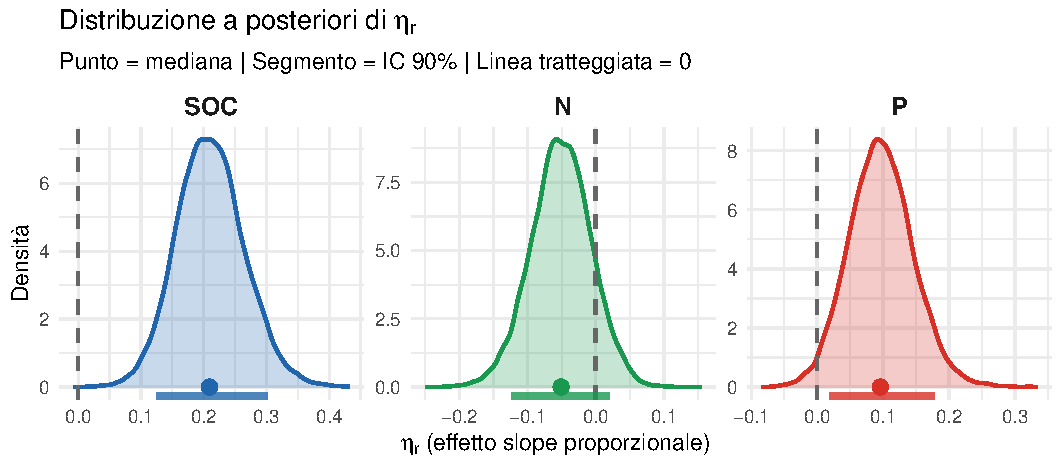
\includegraphics[width=0.8\linewidth]{fig04_eta.pdf}
  \caption{Distribuzioni a posteriori di $\eta_r$ per SOC, N e P.
    La linea tratteggiata indica $\eta = 0$.
    $\hat{\eta}_\SOC = 0.21$ con CI\,90\% $[0.12, 0.30]$ (lontano da zero);
    $\hat{\eta}_N \approx -0.05$ (CI include zero);
    $\hat{\eta}_P = 0.10$ con CI\,90\% $[0.02, 0.18]$ (borderline).}
  \label{fig:eta}
\end{figure}

\begin{table}[htbp]
  \centering
  \caption{Stime a posteriori dei parametri strutturali del modello M-SP.
           Mediana e intervallo credibile al 90\% (CI\,90\%).}
  \label{tab:main}
  \small
  \begin{tabular}{@{}lccc@{}}
    \toprule
    Parametro & SOC & N & P \\
    \midrule
    $\alpha_r$ &
      $-0.240\ \CI{-0.527}{0.049}$ &
      $-2.594\ \CI{-2.800}{-2.381}$ &
      $-2.611\ \CI{-2.959}{-2.257}$ \\[2pt]
    $\psi_r$ &
      $0.323\ \CI{0.231}{0.436}$ &
      $0.197\ \CI{0.131}{0.274}$ &
      $0.392\ \CI{0.293}{0.515}$ \\[2pt]
    $\boldsymbol{\eta_r}$ &
      $\mathbf{0.209}\ \CI{0.125}{0.302}$ &
      $-0.051\ \CI{-0.124}{0.021}$ &
      $0.096\ \CI{0.019}{0.179}$ \\[2pt]
    $b_r = \eta_r/\psi_r$ &
      $0.645\ \CI{0.388}{0.990}$ &
      $-0.252\ \CI{-0.748}{0.103}$ &
      $0.244\ \CI{0.048}{0.461}$ \\[2pt]
    $\sigma_r$ &
      $0.531\ \CI{0.486}{0.582}$ &
      $0.345\ \CI{0.316}{0.378}$ &
      $0.548\ \CI{0.502}{0.599}$ \\
    \bottomrule
  \end{tabular}
\end{table}

\subsection{Effetti fissi within-field (\texorpdfstring{$\gamma_r$}{gamma\_r})}

La Figura~\ref{fig:gamma} e la Tabella~\ref{tab:gamma} mostrano gli effetti
fissi within-field. L'effetto di logBottom è negativo per tutte le risposte
(decadimento con la profondità). Texture2 (ILR$_2$: argilla+limo vs sabbia)
ha un effetto negativo forte per SOC e N: suoli con maggiore contenuto di
argilla tendono ad avere livelli più elevati. BulkDensity è negativa: densità
apparente più alta è associata a minore contenuto organico. Texture1 (ILR$_1$:
argilla vs limo) non è significativamente diverso da zero per nessuna risposta.

\begin{table}[htbp]
  \centering
  \caption{Effetti fissi within-field $\hat{\gamma}_{r,k}$ dal modello M-SP.
           Mediana e CI\,90\%. In grassetto i coefficienti con CI\,90\%
           lontano da zero.}
  \label{tab:gamma}
  \small
  \begin{tabular}{@{}lrrr@{}}
    \toprule
    Covariato & SOC & N & P \\
    \midrule
    logBottom &
      $\mathbf{-0.378}\ [-0.472,\ -0.286]$ &
      $\mathbf{-0.202}\ [-0.253,\ -0.152]$ &
      $-0.062\ [-0.144,\ 0.021]$ \\[2pt]
    Texture1 (ILR$_1$) &
      $-0.055\ [-0.134,\ 0.022]$ &
      $-0.041\ [-0.093,\ 0.011]$ &
      $0.001\ [-0.080,\ 0.082]$ \\[2pt]
    Texture2 (ILR$_2$) &
      $\mathbf{-0.529}\ [-0.660,\ -0.397]$ &
      $\mathbf{-0.288}\ [-0.370,\ -0.205]$ &
      $-0.072\ [-0.215,\ 0.070]$ \\[2pt]
    BulkDensity &
      $\mathbf{-0.223}\ [-0.362,\ -0.084]$ &
      $\mathbf{-0.204}\ [-0.291,\ -0.114]$ &
      $-0.150\ [-0.297,\ -0.001]$ \\
    \bottomrule
    \multicolumn{4}{@{}l}{\small\textit{
      Covariati standardizzati. Texture1 non significativo per nessuna risposta.}} \\
  \end{tabular}
\end{table}

\begin{figure}[htbp]
  \centering
  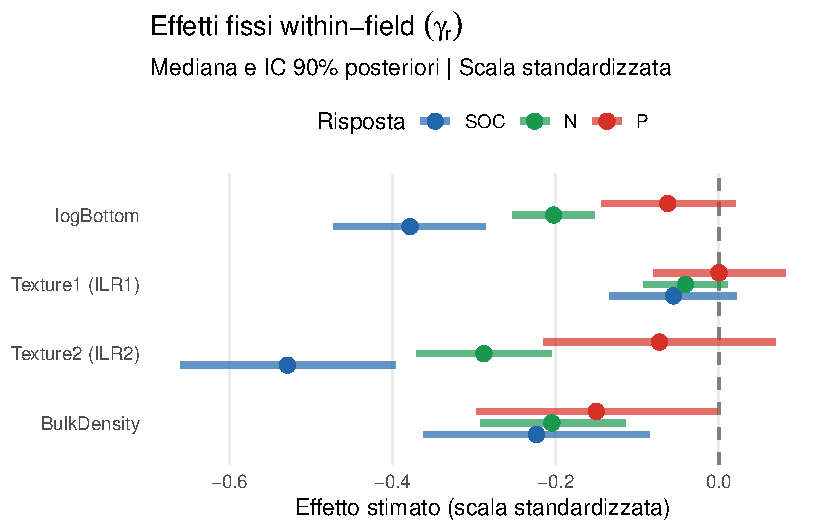
\includegraphics[width=0.8\linewidth]{fig05_gamma.pdf}
  \caption{Forest plot degli effetti fissi within-field $\hat{\gamma}_{r,k}$
    (mediana e CI\,90\%) per SOC (blu), N (verde), P (rosso).
    I valori $\neq 0$ indicano effetti sistematici della tessitura e della
    densità apparente sui profili verticali.}
  \label{fig:gamma}
\end{figure}

\subsection{Posterior predictive check}

La Figura~\ref{fig:ppc} confronta la distribuzione osservata di logSOC, logN
e logP con 100 repliche simulate dal modello a posteriori. Il modello replica
bene la forma delle distribuzioni, senza evidenti discrepanze sistematiche.

\begin{figure}[htbp]
  \centering
  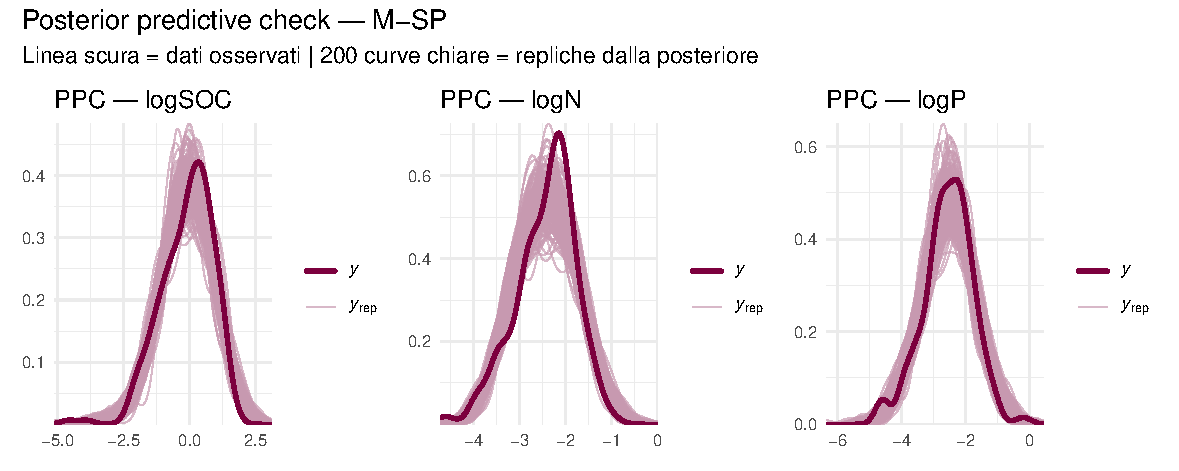
\includegraphics[width=0.8\linewidth]{fig08_ppc.pdf}
  \caption{Posterior predictive check: densità osservata (linea nera spessa)
    vs.\ 100 repliche a posteriori (linee grigie) per le tre risposte.}
  \label{fig:ppc}
\end{figure}

\subsection{Robustezza alle osservazioni influenti}
\label{subsec:sensitivity}

La diagnostica PSIS-LOO identifica 10 osservazioni con Pareto $k \geq 0.7$
(4.5\% del totale; 1 con $k > 1$, da campo~26 a profondità 20~cm).
Il modello M-SP è stato rifittato dopo la rimozione di queste osservazioni.

La Figura~\ref{fig:sensitivity} mostra il confronto di $\eta_r$ tra il modello
completo e il modello senza influenti. I due parametri ATTENZIONE riguardano
$\sigma_\SOC$ (0.531 → 0.440) e $\sigma_N$ (0.345 → 0.266): le osservazioni
influenti sono outlier di residuo che gonfiano la varianza residua.
Le conclusioni su $\eta_r$ sono robuste:
$\eta_\SOC$ rimane chiaramente positivo
($0.209\ [0.125,\,0.302]$ → $0.160\ [0.089,\,0.239]$);
$\eta_N$ rimane vicino a zero in entrambi i casi;
$\eta_P$ è leggermente più forte senza influenti ($0.096$ → $0.119$).

\begin{figure}[htbp]
  \centering
  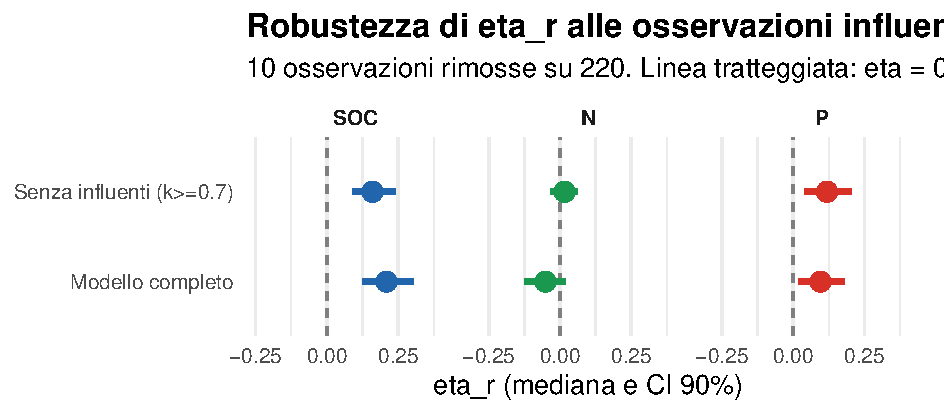
\includegraphics[width=0.8\linewidth]{fig10_sensitivity.pdf}
  \caption{Confronto di $\eta_r$ (mediana e CI\,90\%) tra il modello M-SP
    completo e il modello rifittato dopo rimozione delle 10 osservazioni con
    Pareto $k \geq 0.7$. Le conclusioni sulle tre risposte sono robuste.}
  \label{fig:sensitivity}
\end{figure}


% ==============================================================================
\section{Confronto modelli e selezione variabili}
\label{sec:confronto}

\subsection{Confronto architetturale (LOO-CV)}
\label{subsec:loo4}

La Tabella~\ref{tab:loo4} confronta quattro architetture di modello tramite
LOO-CV \citep{vehtari2017}: M-SP (slope proporzionale, modello finale),
M-RI (solo random intercept), M-GPS (processo gaussiano spaziale + slope fissa)
e M-GP (processo gaussiano completo). La Figura~\ref{fig:loo4} mostra i
$\Delta$ELPD rispetto al migliore.

\begin{figure}[htbp]
  \centering
  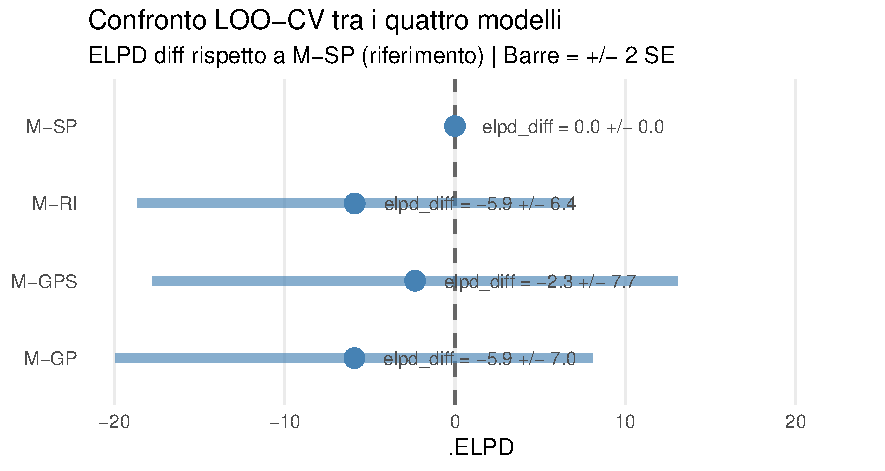
\includegraphics[width=0.8\linewidth]{fig07_loo4.pdf}
  \caption{Confronto LOO-CV dei quattro modelli architetturali.
    M-SP ottiene il miglior ELPD pur avendo meno parametri dei modelli GP.
    L'eterogeneità between-field è catturata dalla slope proporzionale senza
    necessità di un processo gaussiano spaziale.}
  \label{fig:loo4}
\end{figure}

\begin{table}[htbp]
  \centering
  \caption{LOO-CV per i quattro modelli architetturali.
           $\Delta$ELPD rispetto a M-SP; $|z|=|\Delta\text{ELPD}|/\text{SE}$.}
  \label{tab:loo4}
  \small
  \begin{tabular}{@{}llrrr@{}}
    \toprule
    Modello & Descrizione & $\Delta$ELPD & SE & $|z|$ \\
    \midrule
    \textbf{M-SP} & RI + slope proporzionale & $\mathbf{0.0}$ & — & — \\
    M-GPS & GP spaziale + slope fissa  & $-2.3$ & $7.7$ & $0.30$ \\
    M-RI  & Random intercept i.i.d.    & $-5.9$ & $6.4$ & $0.92$ \\
    M-GP  & GP spaziale completo       & $-5.9$ & $7.0$ & $0.84$ \\
    \bottomrule
    \multicolumn{5}{@{}l}{\small\textit{
      $|\Delta\text{ELPD}/\text{SE}| < 2$ per tutti: nessuna differenza significativa.
      M-SP ha il minor numero di parametri effettivi ($p_\text{loo} = 127$).}} \\
  \end{tabular}
\end{table}

\subsection{Selezione variabili (projpred)}

La selezione variabili \emph{projection predictive} \citep{piironen2017}
con M-SP come reference model identifica il sottomodello minimo che non degrada
significativamente la predizione ($\alpha = 0.10$).
La struttura proporzionale (random effect) è sempre inclusa;
la selezione opera sui covariati fissi $\gamma_r$ e $\beta_r$.

\begin{figure}[htbp]
  \centering
  \begin{subfigure}[b]{0.32\linewidth}
    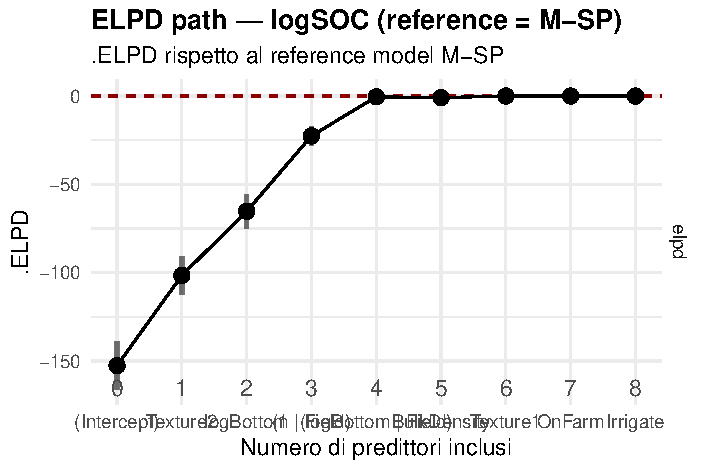
\includegraphics[width=\linewidth]{fig06a_projpred_soc.pdf}
    \caption{SOC}
  \end{subfigure}\hfill
  \begin{subfigure}[b]{0.32\linewidth}
    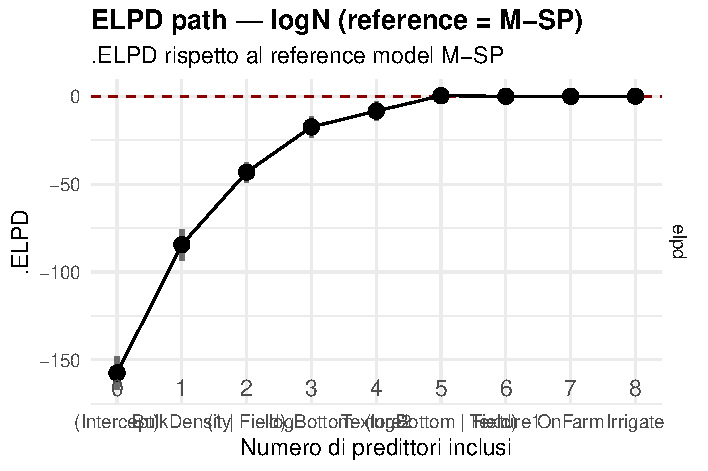
\includegraphics[width=\linewidth]{fig06b_projpred_n.pdf}
    \caption{N}
  \end{subfigure}\hfill
  \begin{subfigure}[b]{0.32\linewidth}
    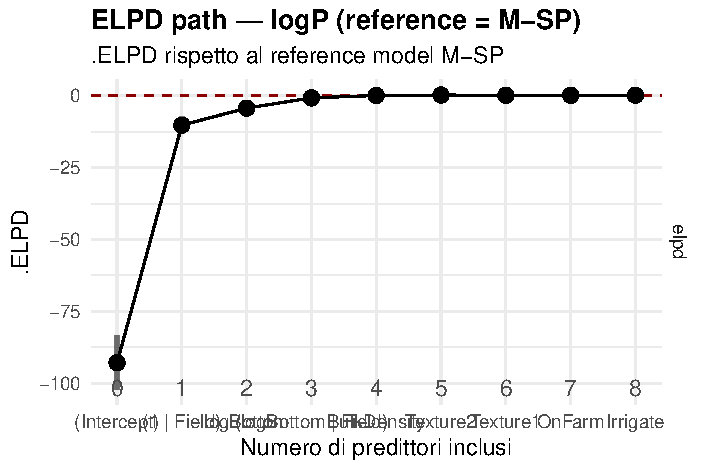
\includegraphics[width=\linewidth]{fig06c_projpred_p.pdf}
    \caption{P}
  \end{subfigure}
  \caption{Percorso di selezione projpred per SOC, N e P.
    Ogni punto mostra $\Delta$ELPD del submodello con $k$ predittori rispetto
    al reference model M-SP. La linea tratteggiata indica la soglia ($\alpha = 0.10$).
    logBottom è sempre incluso; la selezione degli altri predittori è fedele
    al segnale biologico.}
  \label{fig:projpred}
\end{figure}

La Tabella~\ref{tab:projpred} riporta l'ordine di selezione e il numero suggerito
di predittori per ciascuna risposta. Le parentesi indicano termini della struttura
casuale (approssimazione lmer del reference model M-SP); i termini fissi selezionati
corrispondono direttamente ai $\hat{\gamma}_r$ del modello finale.

\begin{table}[htbp]
  \centering
  \caption{Selezione projpred (forward search, PSIS-LOO, $\alpha = 0.10$).
    $n^*$: numero di predittori suggerito. I termini in parentesi indicano
    la struttura random (sempre inclusa nel reference model M-SP).}
  \label{tab:projpred}
  \small
  \begin{tabular}{@{}clp{8.5cm}@{}}
    \toprule
    Risposta & $n^*$ & Ordine di selezione \\
    \midrule
    SOC & 4 &
      Texture2 $\to$ logBottom $\to$ \textit{(1|Field)} $\to$
      \textit{(logBottom|Field)} $\to$ BulkDensity $\to$ \ldots \\[3pt]
    N   & 4 &
      BulkDensity $\to$ \textit{(1|Field)} $\to$ logBottom $\to$ Texture2
      $\to$ \textit{(logBottom|Field)} $\to$ \ldots \\[3pt]
    P   & 3 &
      \textit{(1|Field)} $\to$ logBottom $\to$
      \textit{(logBottom|Field)} $\to$ BulkDensity $\to$ \ldots \\
    \bottomrule
    \multicolumn{3}{@{}p{12cm}}{%
      \small\textit{Effetti fissi selezionati entro $n^*$:
      SOC: \{Texture2, logBottom\};
      N: \{BulkDensity, logBottom, Texture2\};
      P: \{logBottom\}.
      Texture1 e le variabili di management non entrano mai
      nei primi $n^*$ termini.}} \\
  \end{tabular}
\end{table}

La coerenza tra la selezione projpred e il modello M-SP è verificata in due modi.
La Figura~\ref{fig:proj_vs_msp} confronta i coefficienti $\hat{\gamma}_r$ di M-SP
con le posterior proiettate: l'accordo è molto buono per le variabili selezionate.
La Figura~\ref{fig:nonsel_gamma} mostra che per le variabili \emph{non selezionate}
da projpred, i corrispondenti $\hat{\gamma}_r$ in M-SP sono tutti vicini a zero,
confermando retrospettivamente la selezione.

\begin{figure}[htbp]
  \centering
  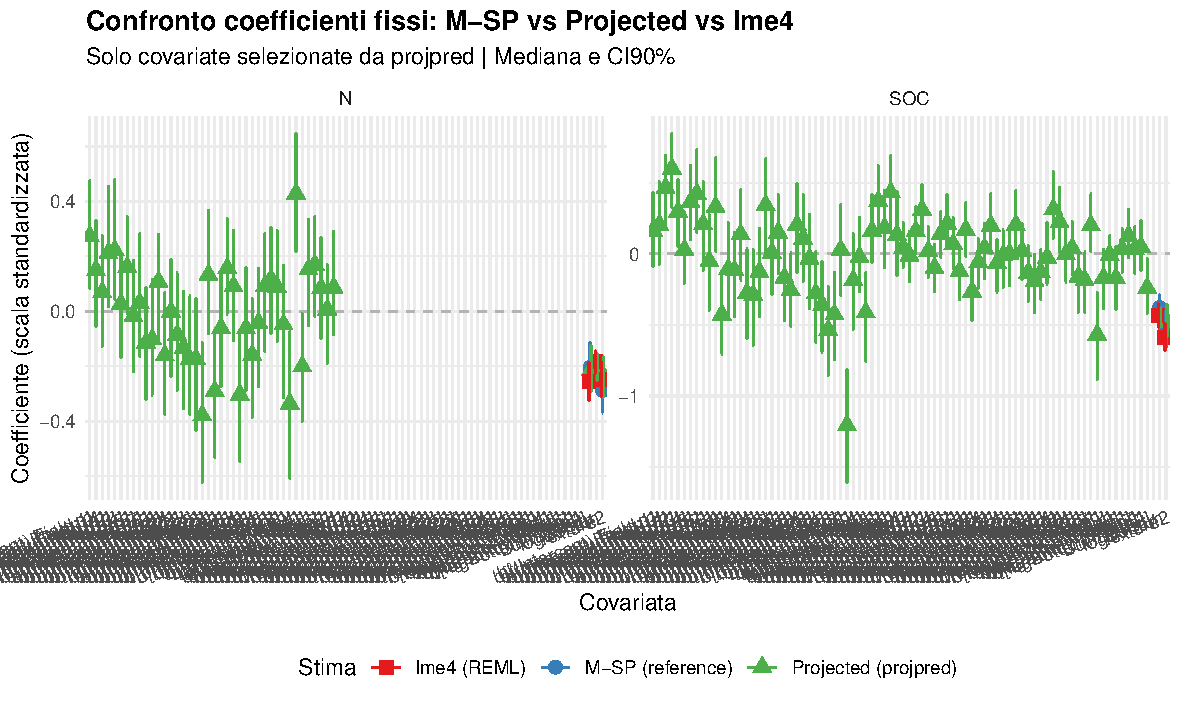
\includegraphics[width=0.8\linewidth]{fig11_proj_vs_msp.pdf}
  \caption{Confronto coefficienti fissi $\hat{\gamma}_r$: modello M-SP (punti)
    vs.\ posterior proiettate via projpred (barre). Accordo sostanziale per tutte
    le variabili selezionate.}
  \label{fig:proj_vs_msp}
\end{figure}

\begin{figure}[htbp]
  \centering
  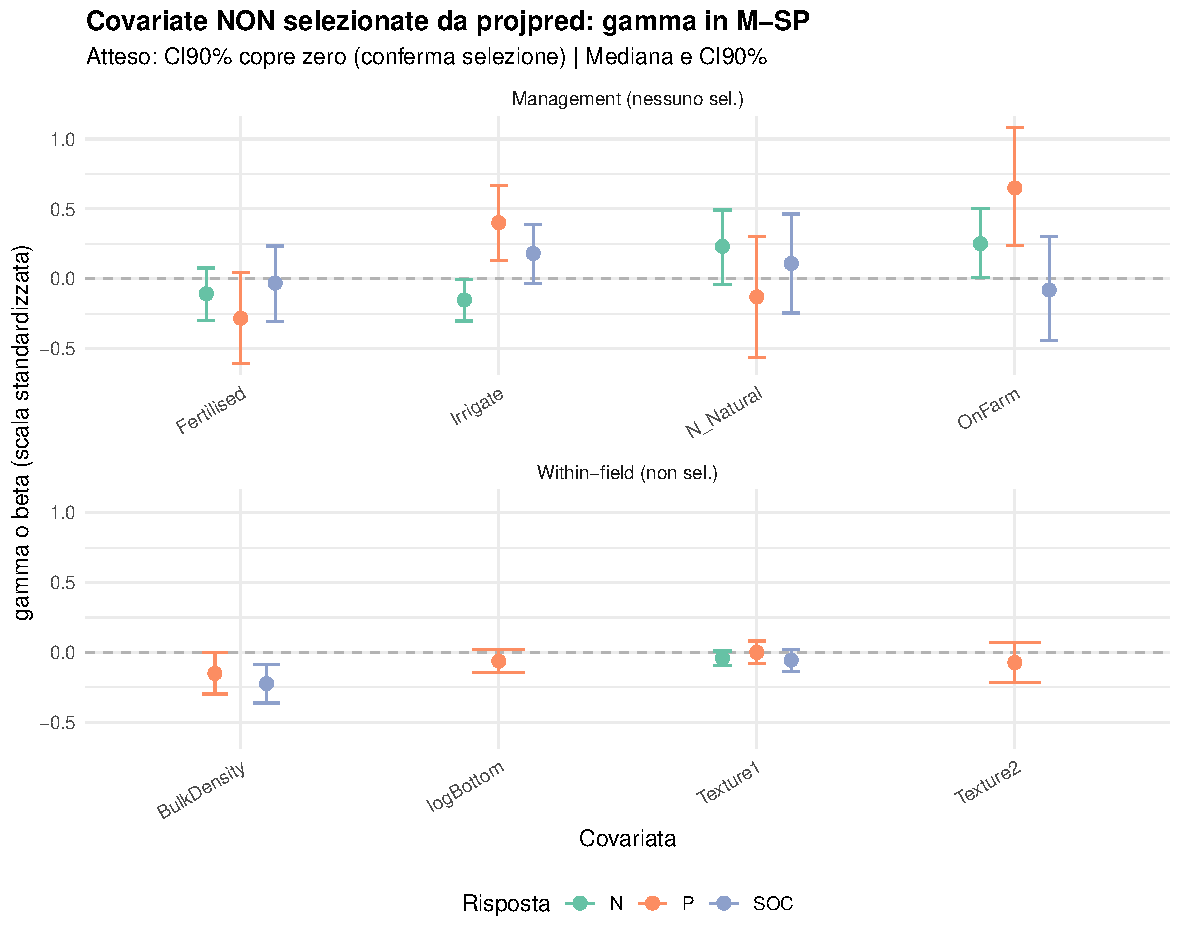
\includegraphics[width=0.8\linewidth]{fig12_nonselected_gamma.pdf}
  \caption{Coefficienti $\hat{\gamma}_r$ per le variabili \emph{non selezionate}
    da projpred in M-SP. Tutti con CI\,90\% compatibili con zero, confermando
    la selezione.}
  \label{fig:nonsel_gamma}
\end{figure}

\subsection{Robustezza alla semplificazione: modelli A e B}

Per verificare che le conclusioni su $\eta_r$ non dipendano dall'inclusione
di variabili non necessarie, sono stati stimati due modelli semplificati:
\begin{itemize}
  \item \textbf{Modello A}: M-SP senza management ($\vec{\beta}_r$ rimosso)
    e senza Texture1, sulla base della selezione projpred.
  \item \textbf{Modello B}: struttura response-specific fedele a projpred
    (N senza slope proporzionale; P con solo logBottom fisso).
\end{itemize}
La Figura~\ref{fig:loo_ab} e la Tabella~\ref{tab:loo_ab} mostrano che tutti e
tre i modelli sono statisticamente indistinguibili in termini predittivi
($|\Delta\text{ELPD}/\text{SE}| < 0.5$). M-SP è preferibile per l'interpretazione
biologica (i $\vec{\beta}_r$ permettono di quantificare gli effetti di management,
anche se deboli).

\begin{figure}[htbp]
  \centering
  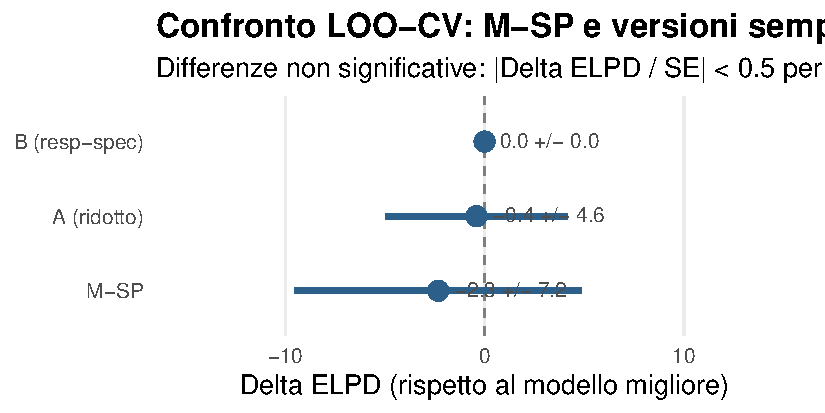
\includegraphics[width=0.8\linewidth]{fig09_loo_ab.pdf}
  \caption{LOO-CV per M-SP, Modello~A (ridotto) e Modello~B (response-specific).
    Le differenze sono nell'ordine del rumore numerico: nessun modello è
    predittivamente superiore.}
  \label{fig:loo_ab}
\end{figure}

\begin{table}[htbp]
  \centering
  \caption{LOO-CV per M-SP e modelli semplificati.
    $\Delta$ELPD rispetto al modello con ELPD più alto (B).}
  \label{tab:loo_ab}
  \small
  \begin{tabular}{@{}llrrr@{}}
    \toprule
    Modello & Descrizione & ELPD & $\Delta$ELPD & SE \\
    \midrule
    B (resp-spec)  & Response-specific & $-504.3$ & $0.0$ & — \\
    A (ridotto)    & M-SP senza X\textsubscript{B} e Texture1 &
                     $-504.7$ & $-0.4$ & $4.6$ \\
    \textbf{M-SP}  & Modello completo  & $-506.7$ & $-2.3$ & $7.2$ \\
    \bottomrule
    \multicolumn{5}{@{}l}{\small\textit{
      Tutti $|\Delta\text{ELPD}/\text{SE}| < 0.5$: differenze non significative.}} \\
  \end{tabular}
\end{table}


% ==============================================================================
\section{Discussione}
\label{sec:discussione}

\subsection{SOC: correlazione slope–intercetta e meccanismi biologici}

Il risultato principale — $\eta_\SOC = 0.21$ chiaramente positivo — indica che
i campi con maggiore SOC alla profondità media mostrano anche un decadimento
più lento con la profondità. Questo pattern è coerente con la letteratura:
\citet{jobbagy2000} riportano che gli strati profondi contribuiscono in modo
sproporzionato agli stock di carbonio nei suoli più ricchi, per effetto della
stabilizzazione organo-minerale e della minore perturbazione meccanica.

% TODO: discussione meccanismi (practices agronomiche che favoriscono
%   sia livelli alti che distribuzione verticale uniforme; radici profonde;
%   BulkDensity come proxy)
% TODO: confronto con Mutambu et al. (2019) e Kirsten et al. (2019)

\subsection{N: profili uniformi tra campi}

$\eta_N \approx 0$ in tutti i modelli testati: la velocità di decadimento
dell'azoto con la profondità non dipende dal livello medio del campo.
Questo risultato è biologicamente plausibile: l'azoto nel suolo è più
mobile del carbonio (mineralizzazione, lisciviazione) e la sua distribuzione
verticale risponde più alle pratiche di fertilizzazione che alla struttura
intrinseca del suolo.

% TODO: riferimenti su mineralizzazione N

\subsection{P: evidenza moderata e dipendenza dalla specificazione}

L'effetto per P è borderline: positivo e lontano da zero in M-SP e A
($\eta_P = 0.096\ [0.019, 0.179]$), ma con CI che include zero nel Modello B
($\eta_P = 0.054\ [-0.016, 0.126]$). La differenza nasce dalla separazione
dell'effetto fisso di logBottom (gamma\_P\_logB in B) da quello casuale
(slope proporzionale). In M-SP le due componenti sono parzialmente
confuse. La conclusione su P deve essere interpretata con cautela.

% TODO: riferimenti su dinamica P nel suolo

\subsection{Effetti di management}

I coefficienti $\vec{\beta}_r$ sono deboli per tutte le risposte (CI\,90\%
che includono lo zero per quasi tutti i termini). Il LOO-CV non mostra
miglioramento dopo la rimozione di X\textsubscript{B} (Modelli A e B).
Questo suggerisce che la variabilità tra campi è catturata
principalmente dalla struttura proporzionale (componente casuale) più
che dalle pratiche agronomiche osservate.

% TODO: riflessione su scale temporali (gli effetti di management richiedono
%   decenni per essere visibili nel profilo verticale)


% ==============================================================================
\section{Conclusioni}
\label{sec:conclusioni}

Questo lavoro ha introdotto e stimato il modello M-SP (slope proporzionale),
un modello bayesiano gerarchico per profili verticali multipli di nutrienti del
suolo. I risultati principali sono:

\begin{enumerate}
  \item \textbf{SOC}: i campi con carbonio organico elevato alla profondità media
    mostrano un decadimento sistematicamente più lento
    ($\hat{\eta}_\SOC = 0.21$, CI\,90\%: $[0.12, 0.30]$). Il risultato è
    robusto alla semplificazione del modello e alla rimozione delle osservazioni
    influenti.
  \item \textbf{N}: non vi è evidenza di una slope proporzionale
    ($\hat{\eta}_N \approx -0.05$, CI include zero). I profili verticali
    dell'azoto sono uniformi tra i campi.
  \item \textbf{P}: evidenza moderata di una slope proporzionale
    ($\hat{\eta}_P = 0.10$, CI\,90\%: $[0.02, 0.18]$ in M-SP), ma il risultato
    è sensibile alla specificazione del modello.
\end{enumerate}

Dal punto di vista metodologico, la struttura proporzionale (singolo parametro
$\eta_r$) cattura la correlazione intercetta–slope con un numero molto ridotto
di parametri, ottenendo il miglior LOO-CV tra tutti i modelli confrontati.
La selezione variabili projpred e la sensitivity analysis PSIS-LOO hanno
validato la robustezza delle conclusioni.

% TODO: implicazioni pratiche per la gestione del suolo in Tanzania


% ==============================================================================
\bibliography{refs}


% ==============================================================================
\appendix

\section{Effetti di management (\texorpdfstring{$\beta_r$}{beta\_r})}
\label{app:beta}

\begin{table}[htbp]
  \centering
  \caption{Effetti di management $\hat{\beta}_{r,k}$ dal modello M-SP
    (mediana e CI\,90\%). Quasi tutti i CI includono zero.}
  \label{tab:beta}
  \small
  \begin{tabular}{@{}lrrr@{}}
    \toprule
    Covariato & SOC & N & P \\
    \midrule
    OnFarm     &
      $-0.081\ [-0.443,\ 0.304]$ &
      $0.251\ [0.009,\ 0.500]$ &
      $0.650\ [0.235,\ 1.080]$ \\[2pt]
    Irrigate   &
      $0.181\ [-0.033,\ 0.388]$ &
      $-0.152\ [-0.303,\ -0.006]$ &
      $0.401\ [0.131,\ 0.665]$ \\[2pt]
    Fertilised &
      $-0.032\ [-0.307,\ 0.234]$ &
      $-0.108\ [-0.300,\ 0.076]$ &
      $-0.283\ [-0.605,\ 0.047]$ \\[2pt]
    N\_Natural  &
      $0.109\ [-0.245,\ 0.463]$ &
      $0.232\ [-0.039,\ 0.492]$ &
      $-0.129\ [-0.564,\ 0.302]$ \\
    \bottomrule
    \multicolumn{4}{@{}p{12cm}}{\small\textit{
      Covariati standardizzati. P mostra effetti più grandi ma con CI ampi.
      Il LOO-CV dei modelli A e B (senza $\vec{\beta}_r$) è statisticamente
      equivalente a M-SP, confermando che il management ha impatto predittivo
      trascurabile.}} \\
  \end{tabular}
\end{table}

\begin{figure}[htbp]
  \centering
  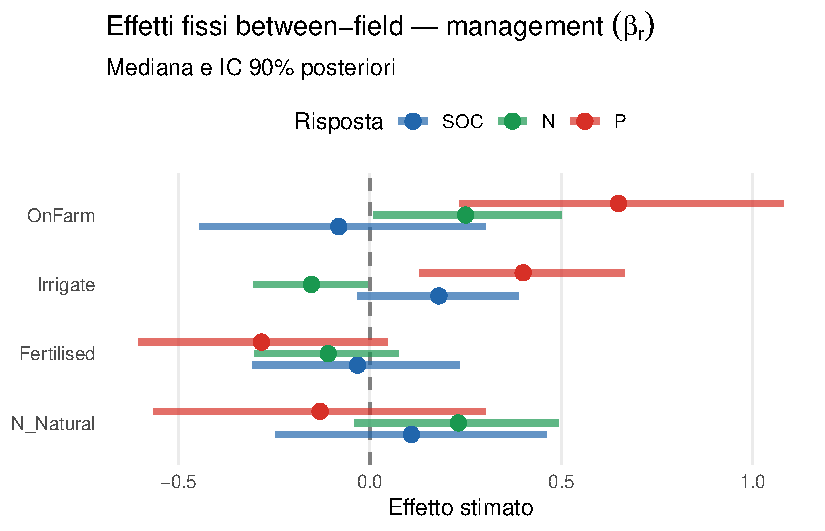
\includegraphics[width=0.8\linewidth]{appfig01_beta.pdf}
  \caption{Forest plot degli effetti di management $\hat{\beta}_{r,k}$ (mediana
    e CI\,90\%). Tutti i coefficienti hanno CI\,90\% che includono lo zero
    o sono di piccola entità pratica.}
  \label{fig:beta}
\end{figure}

\section{Trace plot dei parametri chiave}
\label{app:trace}

\begin{figure}[htbp]
  \centering
  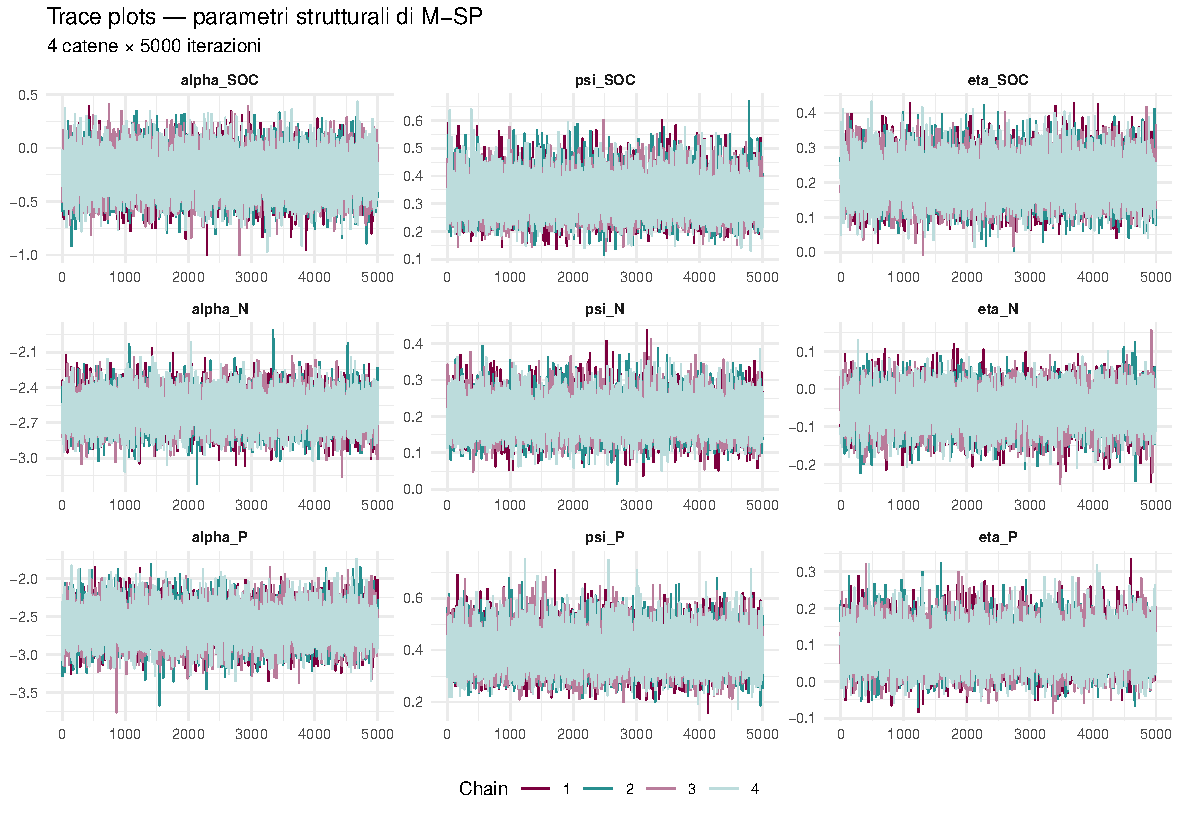
\includegraphics[width=0.8\linewidth]{appfig02_trace.pdf}
  \caption{Trace plot delle 4 catene MCMC per i parametri strutturali
    chiave ($\alpha_r$, $\psi_r$, $\eta_r$ per SOC, N, P).
    Le catene si mescolano bene: nessuna evidenza di mancata convergenza.}
  \label{fig:trace}
\end{figure}

\end{document}
